\exercise{Grundlagen}
Answer the following questions:
\begin{enumerate}
    \item In general, we can distinguish between two forms of machine learning.
    Which are these and how can we characterize them?
    \item Which traditional forms of machine learning do you know?
    \item Define the following terms:
    Hyperparameter, Bias, Classifier, Dataset, Clustering, Loss-Function, Class, Parameter, Datapoint, Variance, Regression, Training
\end{enumerate}
%
%
\exercise{Traditional Machine Learning Procedures}
Familiarize yourself with the provided script \mintinline{bash}{polynomial_fit.ipynb}.
Discuss strengths and weaknesses of the methods shown.
%
%
\section*{Understanding Neural Networks}
Let $x=(x_1,\dots,x_n)$ be the input vector und $g(x)=(g(x)_1,\dots,g(x)_m)$ the output vector of a neural network.
We denote the loss function (Cost-Funktion) with $C$ and with $L$ the number of layers.
The weights between layer $l-1$ and $l$ and between node $j$ of layer $l$ and node $k$ of layer $l-1$ are written as $W^l=w^l_{jk}$.
The number of nodes per layer $l$ is given by $\sigma_l$.
Figure~\ref{neural-network} shows an example for such a neural network.
\begin{figure}[htp]
    \centering
    \tikzset{%
        every neuron/.style={
            circle,
            draw,
            minimum size=1cm
        },
        neuron missing/.style={
            draw=none, 
            scale=3,
            text height=0.333cm,
            execute at begin node=\color{black}$\vdots$
        },
    }
    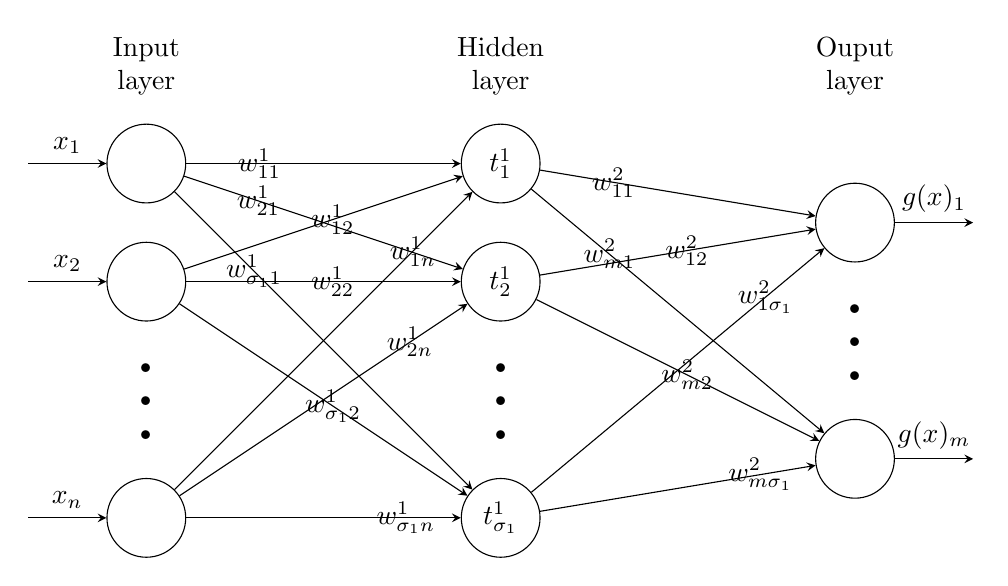
\begin{tikzpicture}[x=1.5cm, y=1.5cm, >=stealth]

        \foreach \m/\l [count=\y] in {1,2,missing,3}
        \node [every neuron/.try, neuron \m/.try] (input-\m) at (0,2-\y) {};

        \foreach \m [count=\y] in {1,2,missing,3}
        \node [every neuron/.try, neuron \m/.try ] (hidden-\m) at (3,2-\y) {\ifnum\y=3\else \ifnum\y=4 $t^1_{\sigma_1}$\else$t^1_{\m}$\fi\fi};

        \foreach \m [count=\y] in {1,missing,2}
        \node [every neuron/.try, neuron \m/.try ] (output-\m) at (6,1.5-\y) {};

        \foreach \l [count=\i] in {1,2,n}
        \draw [<-] (input-\i) -- ++(-1,0)
            node [above, midway] {$x_\l$};

        \foreach \l [count=\i] in {1,m}
        \draw [->] (output-\i) -- ++(1,0)
            node [above, midway] {$g(x)_\l$};

        \foreach \i [count=\l] in {1,2,n}
        \foreach \j [count=\k] in {1,2,\sigma_1}
            \draw [->] (input-\l) -- (hidden-\k)
                node [pos=0.8*\l/3] {$w^1_{\j\i}$};
        
        \foreach \i [count=\l] in {1,2,\sigma_1}
        \foreach \j [count=\k] in {1,m}
            \draw [->] (hidden-\l) -- (output-\k)
                node [pos=0.8*\l/3] {$w^2_{\j\i}$};

        \foreach \l [count=\x from 0] in {Input, Hidden, Ouput}
        \node [align=center, above] at (\x*3,1.5) {\l \\ layer};
    \end{tikzpicture}
    \caption{Example of a neural network with only one hidden layer.}
    \label{neural-network}
\end{figure}
The total function $g$ of the layer can be split along the function of the individual layers $f^l$.
We can thus write
\begin{equation}
    g(x) = f^L(W^Lf^{L-1}(W^{L-1}\dots f^1(W^1x)\dots))
\end{equation}
We inspect the first layer of our example in figure~\ref{neural-network}.
Here, the result at the first hidden layer will be
\begin{align}
    t^1_j &= f^1\left(w^1_{j1}x_1 + w^1_{j2}x_2 + \dots + w^1_{jn}x_n\right)\\
    t^1_j &= f^1\left(\sum\limits_{k=0}^n w^1_{jk}x_k\right)
\end{align}
or generally speaking for a larger neural network
\begin{equation}
    t^{l+1}_j = f^{l+1}\left(\sum\limits_{k=0}^{\sigma_{l}} w^{l+1}_{jk} t^{l}_k\right).
\end{equation}
\exercise{Building Neural Networks}
\begin{enumerate}
    \item Build a neural network with one input node and one output node and no hidden layers.
    We fix the 
    This network should return double its input value.
\end{enumerate}
